% !TeX root = ../../main.tex

\subsection{RoboReacher Gym Environment: Multi-Agent Distributed Experiment}

Since the distributed setup achieve higher performance, we will be moving to a more higher and complex distributed algorithms which provides high performance throughput and can scale to support multi-agent environments and simulate in a larger scale for achieving faster training and performance in the least amount of time providing a high performance computing power.

\subsubsection{Aim of the experiment}
% 1. Question behind (in the heading, why interesting, what to investigate)

This experiment is designed to be performed on large multi-agents scale in distributed setup using APE-X DDPG Algorithm for continuous spaces. Using a single GPU learner and many CPU workers for experience collection. Experience collection can scale to hundreds of CPU workers due to the distributed prioritization of experience prior to storage in replay buffers.

We want to investigate how the agent will perform in the experiment, the time taken to run the experiment, the average episode reward the agent will get and whether the agent will be able to solve the environment in a constrained stopping conditions.

\subsubsection{Setup and configurations}

In this experiment, Distributed Prioritized Experience Replay (Ape-X) algorithm is selected to train the agents in the experiments. Since this experiment is Scalable Multi-Agent, the experiment was performed with multiple number of agents and environment per each agent to test the Scalability and efficiency and determine the best setup for the experiment.

Below are the default configuration for Ape-X algorithm:
\lstinputlisting[language=Python]{chapters/04/apex_default.py}

followed by this experiment setup and configuration as listed below:
\begin{table}[!htb]
    \centering
    \begin{tabular}{|c|l|l|c|l|l|}
    \hline
    \multicolumn{6}{|c|}{\textit{\textbf{Gym Reacher Ape-X 3rd Experiment: Multi-Agent Distributed Experiment}}}                                                        \\ \hline
    \multicolumn{3}{|c|}{\textbf{env}}                                  & \multicolumn{3}{c|}{RoboschoolReacher-v1}                                           \\ \hline
    \multicolumn{3}{|c|}{\textbf{env\_type}}                            & \multicolumn{3}{c|}{OpenAI Environment}                                             \\ \hline
    \multicolumn{3}{|c|}{\textbf{run: Algorithms}}                      & \multicolumn{3}{c|}{\cellcolor[HTML]{C0C0C0}\textbf{APEX\_DDPG}}                           \\ \hline
    \multicolumn{3}{|c|}{}                                              & \multicolumn{3}{c|}{\cellcolor[HTML]{E1F7E1}episode\_reward\_mean = 21}             \\ \cline{4-6} 
    \multicolumn{3}{|c|}{\multirow{-2}{*}{\textbf{stop condition}}}     & \multicolumn{3}{c|}{\cellcolor[HTML]{E1F7E1}time-steps\_total = 10000000: 10M Steps} \\ \hline
    \multicolumn{3}{|c|}{\textbf{use\_huber}}                                & \multicolumn{3}{c|}{True}                                                           \\ \hline
    \multicolumn{3}{|c|}{\textbf{clip\_rewards}}                            & \multicolumn{3}{c|}{False}                                                            \\ \hline
    \multicolumn{3}{|c|}{\textbf{n\_step}}                       & \multicolumn{3}{c|}{3}                                                             \\ \hline
    \multicolumn{3}{|c|}{\textbf{exploration\_ou\_noise\_scale}}                                   & \multicolumn{3}{c|}{1.0}                                                         \\ \hline
    \multicolumn{3}{|c|}{\textbf{target\_network\_update\_freq}}                 & \multicolumn{3}{c|}{50000}                                                           \\ \hline
    \multicolumn{3}{|c|}{\textbf{tau}}                   & \multicolumn{3}{c|}{1.0}                                                          \\ \hline
    \multicolumn{3}{|c|}{\textbf{evaluation\_interval}}                          & \multicolumn{3}{c|}{5}                                             \\ \hline
    \multicolumn{3}{|c|}{\textbf{evaluation\_num\_episodes}}                  & \multicolumn{3}{c|}{MeanStdFilter}                                                  \\ \hline
    \multicolumn{3}{|c|}{\cellcolor[HTML]{C0C0C0}\textbf{num\_gpus}}    & \multicolumn{3}{c|}{\cellcolor[HTML]{C0C0C0}1}                                      \\ \hline
    \multicolumn{3}{|c|}{\cellcolor[HTML]{C0C0C0}\textbf{num\_workers}} & \multicolumn{3}{c|}{\cellcolor[HTML]{C0C0C0}11}                                      \\ \hline
    \multicolumn{3}{|c|}{\cellcolor[HTML]{C0C0C0}\textbf{num\_envs\_per\_worker}} & \multicolumn{3}{c|}{\cellcolor[HTML]{C0C0C0}grid\_search: [32, 16]}                                      \\ \hline
    \end{tabular}
    \caption{Gym Reacher Ape-X 3rd Experiment: Multi-Agent Distributed Experiment}
    \label{tab:gym_reacher_apex_3rd_exp}
\end{table}

As shown in the configuration table~\ref{tab:gym_reacher_apex_3rd_exp} above, we setup the number of environments to be for the first time 32 per each worker leading the experiment to have 384 parallel environment running in the experiment. The second run of the experiment have 16 environment per worker, in this way the experiment have 192 environment running in the experiment. The number of the environment can be much bigger that this in there are more powerful computing provided.


\subsubsection{Experiment Results}

The experiment is performed until an average reward of 21 achieved or for a maximum of 10000000 (10M) steps if no improvement is observable. For evaluating the model performance, we compare the average reward between both experiments. In total, we measure the following metrics averaging over each episode:
\begin{itemize}
    \item The Maximum reward the agent can achieve
    \item The Average reward the agent can achieve
    \item The Minimum reward the agent can achieve
    \item The Total Time Steps obtained by the agent
    \item The Total loss for the selected algorithm
    % \item The Policy loss of the algorithm
    % \item The Value function loss of the algorithm
    % \item The Environment wait time in milliseconds
    \item The Total Time taken to perform the experiment
\end{itemize}

Starting from the maximum reward the agent has obtained, we observe that the agent could quickly learn how to reach the target sphere after only 1M time-steps, passing the non-distributed agent score. After 4M time-steps, the agent achieve the maximum reward (40) that can be obtained in the environment. In the following figure~\ref{fig:2nd_exp_max_eps_reward}, the performance of both the agent for the maximum reward in the environment is shown below:
\begin{figure}[!htb]
    \centering
    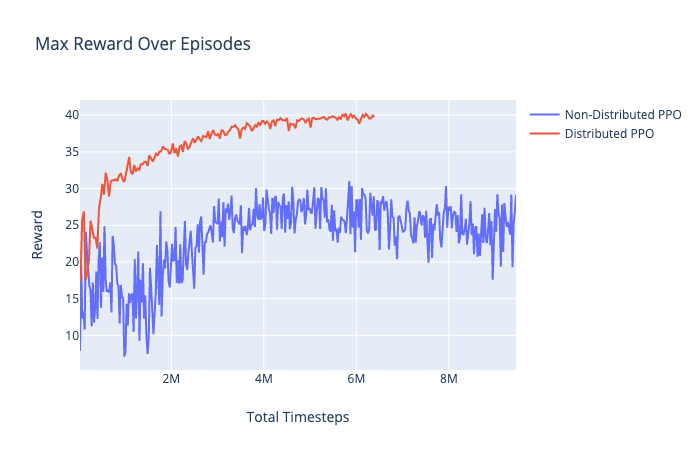
\includegraphics[width=\linewidth]{figures/exps/2nd_exp/max_eps_reward.png}
    \caption{Maximum Reward over Episodes}
    \label{fig:2nd_exp_max_eps_reward}
\end{figure}

Since the experiments are constrained under the conditions of reaching average reward of 21 or completing 10M steps, we compare the performance of both agents for the average reward. The observation are the distributed version of the agent exceed the average reward obtained by the non-distributed agent after only 500,000 time-steps. Followed by performance improvement over time-steps as the agent reach 15 reward after 2M time-steps, and reaching 20 reward after 4M time-steps, leading the agent to solve the environment and achieve the specified 21 average reward after 6M time-steps only. Hence, the agent performance is better than the previous one and could solve the environment effectively before reaching 10M time-steps. The following figure~\ref{fig:2nd_exp_avg_eps_reward}, illustrate the performance of each agent for obtaining the average rewards.
\begin{figure}[!htb]
    \centering
    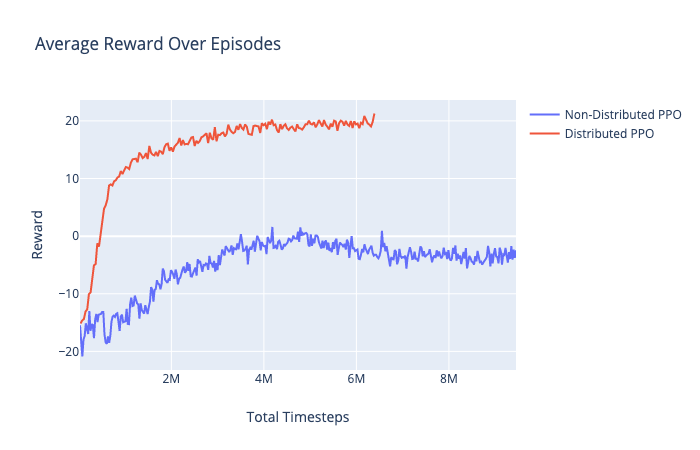
\includegraphics[width=\linewidth]{figures/exps/2nd_exp/avg_eps_reward.png}
    \caption{Maximum Reward over Episodes}
    \label{fig:2nd_exp_avg_eps_reward}
\end{figure}

Comparing the losses of both experiments, we observe the huge decrease and stability of the Distributed PPO total loss after 500,000 time-steps and reaching approximately 0 after 2M time-steps. In contrast with the non-distributed PPO, which shows a high variance in the total loss between 7 and 3 values and never reaching zero as shown in the following figure~\ref{fig:2nd_exp_total_loss}
\begin{figure}[!htb]
    \centering
    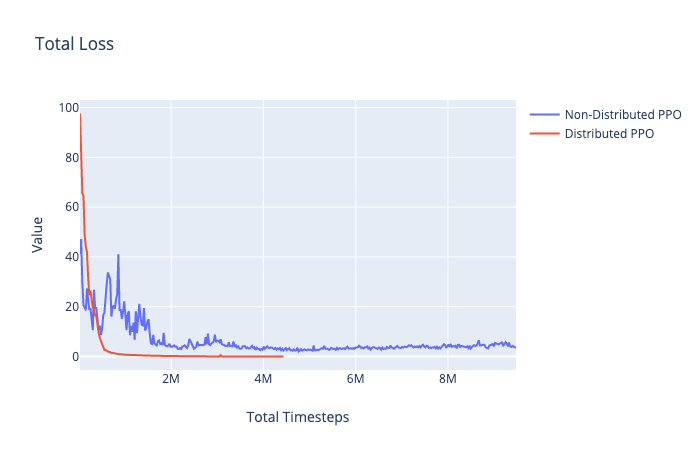
\includegraphics[width=\linewidth]{figures/exps/2nd_exp/total_loss.png}
    \caption{Total Loss}
    \label{fig:2nd_exp_total_loss}
\end{figure}

Comparing between the experiment's total taken time is crucial as it's one of the main key concept for our experiments. Running the two experiments multiple times with different seeds, we observe that the distributed experiment take half the time needed to perform the non-distributed experiment, making it much faster to train and execute reinforcement learning algorithms in distributed setup. The following figure~\ref{fig:2nd_exp_total_training_time} show the time taken for each experiment per hour.
\begin{figure}[!htb]
    \centering
    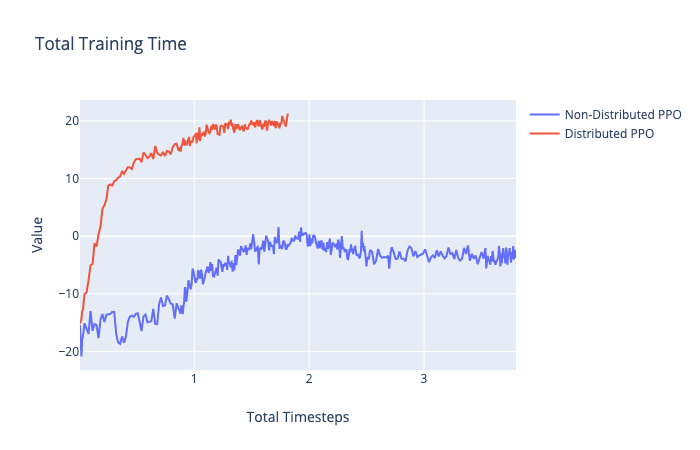
\includegraphics[width=\linewidth]{figures/exps/2nd_exp/total_training_time.png}
    \caption{Total Training Time}
    \label{fig:2nd_exp_total_training_time}
\end{figure}


\subsubsection{Conclusion}

In this experiment, we perform a training and evaluation for the robotic arm using distributed version of ppo algorithm to train our agent. As shown in the results, we conclude that the distributed experiment is much better than the non-distributed version in the training time, the learning process for the agent and for solving the required task.